\graphicspath{ {images/} }

\titledquestion{Analyzing NMT Systems}[25]

\begin{parts}

    \part[3] Look at the {\monofam{src.vocab}} file for some examples of phrases and words in the source language vocabulary. When encoding an input Mandarin Chinese sequence into ``pieces'' in the vocabulary, the tokenizer maps the sequence to a series of vocabulary items, each consisting of one or more characters (thanks to the {\monofam{sentencepiece}} tokenizer, we can perform this segmentation even when the original text has no white space). Given this information, how could adding a 1D Convolutional layer after the embedding layer and before passing the embeddings into the bidirectional encoder help our NMT system? \textbf{Hint:} each Mandarin Chinese character is either an entire word or a morpheme in a word. Look up the meanings of 电, 脑, and 电脑 separately for an example. The characters 电 (electricity) and  脑 (brain) when combined into the phrase 电脑 mean computer.

\ifans{
Running a convolutional layer helps us to extract features from neighbors correlated symbols. This way we can help the network to extract the composed meaning of symbols placed next to each other.
}

    \part[8] Here we present a series of errors we found in the outputs of our NMT model (which is the same as the one you just trained). For each example of a reference (i.e., `gold') English translation, and NMT (i.e., `model') English translation, please:
    
    \begin{enumerate}
        \item Identify the error in the NMT translation.
        \item Provide possible reason(s) why the model may have made the error (either due to a specific linguistic construct or a specific model limitation).
        \item Describe one possible way we might alter the NMT system to fix the observed error. There are more than one possible fixes for an error. For example, it could be tweaking the size of the hidden layers or changing the attention mechanism.
    \end{enumerate}
    
    Below are the translations that you should analyze as described above. Only analyze the underlined error in each sentence. Rest assured that you don't need to know Mandarin to answer these questions. You just need to know English! If, however, you would like some additional color on the source sentences, feel free to use a resource like \url{https://www.archchinese.com/chinese_english_dictionary.html} to look up words. Feel free to search the training data file to have a better sense of how often certain characters occur.

    \begin{subparts}
        \subpart[2]
        \textbf{Source Sentence:} 贼人其后被警方拘捕及被判处盗窃罪名成立。 \newline
        \textbf{Reference Translation:} \textit{\underline{the culprits were} subsequently arrested and convicted.}\newline
        \textbf{NMT Translation:} \textit{\underline{the culprit was} subsequently arrested and sentenced to theft.}
        
\ifans{
\begin{enumerate}
    \item In this case the error is that the subject identified by NMT is a singular person while the true translation is plural. Regardless this error, the model identified correctly the verb auxiliary.
    \item This may be due to the number of times that the singular form appears in the training corpus compared to the plural form
    \item One possible solution might be increasing the corpus size and including more examples of the plural forms of the words.
\end{enumerate}
}

        \subpart[2]
        \textbf{Source Sentence}: 几乎已经没有地方容纳这些人,资源已经用尽。\newline
        \textbf{Reference Translation}: \textit{there is almost no space to accommodate these people, and resources have run out.   }\newline
        \textbf{NMT Translation}: \textit{the resources have been exhausted and \underline{resources have been exhausted}.}
        
\ifans{
\begin{enumerate}
    \item In this case the model has hallucinated and omitted a complete part of the sentence.
    \item This seems to be caused by the length of the sentence and the loss of relationship between the last words and the initial ones in the decoder (i.e. the loss of relationship between the initial and subsequent hidden states for long sentences).
    \item One possible solution might be to add an attention output not only between the last word and the encoder states but also with the different previous decoder states.
\end{enumerate}
}        

        \subpart[2]
        \textbf{Source Sentence}: 当局已经宣布今天是国殇日。 \newline
        \textbf{Reference Translation}: \textit{authorities have announced \underline{a national mourning today.}}\newline
        \textbf{NMT Translation}: \textit{the administration has announced \underline{today's day.}}
        
\ifans{ 
\begin{enumerate}
    \item In this case the model failed to capture the meaning of a national mourning day.
    \item This seems to be caused by the absence of enough data in the training corpus and maybe because the usual construction in english is "a national day of mourning" which is different than "a national mourning".
    \item One possible solution might be to add more examples of this kind of constructions in the corpus.
\end{enumerate}
} 
        
        \subpart[2] 
        \textbf{Source Sentence\footnote{This is a Cantonese sentence! The data used in this assignment comes from GALE Phase 3, which is a compilation of news written in simplified Chinese from various sources scraped from the internet along with their translations. For more details, see \url{https://catalog.ldc.upenn.edu/LDC2017T02}. }:} 俗语有云:``唔做唔错"。\newline
        \textbf{Reference Translation:} \textit{\underline{`` act not, err not "}, so a saying goes.}\newline
        \textbf{NMT Translation:} \textit{as the saying goes, \underline{`` it's not wrong. "}}

\ifans{ 
\begin{enumerate}
    \item In this case the model misinterprets the quote.
    \item This may be caused because quotes in different languages are expressed in different manners. In this case the model may have tried to do a hard translation without having context of typical quotes in the source language.
    \item One possible solution might be to add more examples of quotes in the corpus and also improve the attention score to take into account the quotation marks to identify that the sentence is a quote and should not be translated with a direct translation.
\end{enumerate}
} 
        
    \end{subparts}


    \part[14] BLEU score is the most commonly used automatic evaluation metric for NMT systems. It is usually calculated across the entire test set, but here we will consider BLEU defined for a single example.\footnote{This definition of sentence-level BLEU score matches the \texttt{sentence\_bleu()} function in the \texttt{nltk} Python package. Note that the NLTK function is sensitive to capitalization. In this question, all text is lowercased, so capitalization is irrelevant. \\ \url{http://www.nltk.org/api/nltk.translate.html\#nltk.translate.bleu_score.sentence_bleu}
    } 
    Suppose we have a source sentence $\bs$, a set of $k$ reference translations $\br_1,\dots,\br_k$, and a candidate translation $\bc$. To compute the BLEU score of $\bc$, we first compute the \textit{modified $n$-gram precision} $p_n$ of $\bc$, for each of $n=1,2,3,4$, where $n$ is the $n$ in \href{https://en.wikipedia.org/wiki/N-gram}{n-gram}:
    \begin{align}
        p_n = \frac{ \displaystyle \sum_{\text{ngram} \in \bc} \min \bigg( \max_{i=1,\dots,k} \text{Count}_{\br_i}(\text{ngram}), \enspace \text{Count}_{\bc}(\text{ngram}) \bigg) }{\displaystyle \sum_{\text{ngram}\in \bc} \text{Count}_{\bc}(\text{ngram})}
    \end{align}
     Here, for each of the $n$-grams that appear in the candidate translation $\bc$, we count the maximum number of times it appears in any one reference translation, capped by the number of times it appears in $\bc$ (this is the numerator). We divide this by the number of $n$-grams in $\bc$ (denominator). \newline 

    Next, we compute the \textit{brevity penalty} BP. Let $len(c)$ be the length of $\bc$ and let $len(r)$ be the length of the reference translation that is closest to $len(c)$ (in the case of two equally-close reference translation lengths, choose $len(r)$ as the shorter one). 
    \begin{align}
        BP = 
        \begin{cases}
            1 & \text{if } len(c) \ge len(r) \\
            \exp \big( 1 - \frac{len(r)}{len(c)} \big) & \text{otherwise}
        \end{cases}
    \end{align}
    Lastly, the BLEU score for candidate $\bc$ with respect to $\br_1,\dots,\br_k$ is:
    \begin{align}
        BLEU = BP \times \exp \Big( \sum_{n=1}^4 \lambda_n \log p_n \Big)
    \end{align}
    where $\lambda_1,\lambda_2,\lambda_3,\lambda_4$ are weights that sum to 1. The $\log$ here is natural log.
    \newline
    \begin{subparts}
        \subpart[5] Please consider this example: \newline
        Source Sentence $\bs$: \textbf{需要有充足和可预测的资源。} 
        \newline
        Reference Translation $\br_1$: \textit{resources have to be sufficient and they have to be predictable}
        \newline
        Reference Translation $\br_2$: \textit{adequate and predictable resources are required}
        
        NMT Translation $\bc_1$: there is a need for adequate and predictable resources
        
        NMT Translation $\bc_2$: resources be sufficient and predictable to
        
        Please compute the BLEU scores for $\bc_1$ and $\bc_2$. Let $\lambda_i=0.5$ for $i\in\{1,2\}$ and $\lambda_i=0$ for $i\in\{3,4\}$ (\textbf{this means we ignore 3-grams and 4-grams}, i.e., don't compute $p_3$ or $p_4$). When computing BLEU scores, show your work (i.e., show your computed values for $p_1$, $p_2$, $len(c)$, $len(r)$ and $BP$). Note that the BLEU scores can be expressed between 0 and 1 or between 0 and 100. The code is using the 0 to 100 scale while in this question we are using the \textbf{0 to 1} scale. Please round your responses to 3 decimal places. 
        \newline
        
        Which of the two NMT translations is considered the better translation according to the BLEU Score? Do you agree that it is the better translation?
        
\ifans{
\begin{itemize}
    \item For c1:
    \begin{gather*}
        p_1 = \frac{0 + 0 + 0 + 0 + 0 + 1 + 1 + 1 + 1}{9} = \frac{4}{9} \\
        p_2 = \frac{0 + 0 + 0 + 0 + 0 + 1 + 1 + 1}{8} = \frac{3}{8} \\
        len(c1) = 9 \\
        len(r1) = 11 \\
        len(r2) = 6 \\
        BP = \exp ( 1 - \frac{11}{9}) \\
        BLEU = \exp ( 1 - \frac{11}{9}) \times \exp ( 0.5 \times log(\frac{4}{9}) + 0.5 \times log(\frac{3}{8})) \approx 0.327
    \end{gather*}
    
    \item For c2:
    \begin{gather*}
        p_1 = \frac{1 + 1 + 1 + 1 + 1 + 1}{6} = 1 \\
        p_2 = \frac{0 + 1 + 1 + 1 + 0}{5} = \frac{3}{5} \\
        len(c2) = 6 \\
        len(r1) = 11 \\
        len(r2) = 6 \\
        BP = 1 \\
        BLEU = 1 \times \exp ( 0.5 \times log(1) + 0.5 \times log(\frac{3}{5})) \approx 0.775
    \end{gather*}
\end{itemize}
According to the BLEU score, the second translation (c2) is better than the first one (c1). I'm not agree with this conclusion, since the first translation captures better the idea of the sentence.
}
        
        \subpart[5] Our hard drive was corrupted and we lost Reference Translation $\br_1$. Please recompute BLEU scores for $\bc_1$ and $\bc_2$, this time with respect to $\br_2$ only. Which of the two NMT translations now receives the higher BLEU score? Do you agree that it is the better translation?

\ifans{
\begin{itemize}
    \item For c1:
    \begin{gather*}
        p_1 = \frac{0 + 0 + 0 + 0 + 0 + 1 + 1 + 1 + 1}{9} = \frac{4}{9} \\
        p_2 = \frac{0 + 0 + 0 + 0 + 0 + 1 + 1 + 1}{8} = \frac{3}{8} \\
        len(c1) = 9 \\
        len(r2) = 6 \\
        BP = 1 \\
        BLEU = 1 \times \exp ( 0.5 \times log(\frac{4}{9}) + 0.5 \times log(\frac{3}{8})) \approx 0.408
    \end{gather*}
    
    \item For c2:
    \begin{gather*}
        p_1 = \frac{1 + 0 + 0 + 1 + 1 + 0}{6} = \frac{3}{6} \\
        p_2 = \frac{0 + 0 + 0 + 1 + 0}{5} = \frac{1}{5} \\
        len(c2) = 6 \\
        len(r2) = 6 \\
        BP = 1 \\
        BLEU = 1 \times \exp ( 0.5 \times log(\frac{3}{6}) + 0.5 \times log(\frac{1}{5})) \approx 0.316 
    \end{gather*}
\end{itemize}
According to this BLEU score, the first translation (c1) is better than the second one (c2). I'm agree with this conclusion.
}
        
        
        \subpart[2] Due to data availability, NMT systems are often evaluated with respect to only a single reference translation. Please explain (in a few sentences) why this may be problematic. In your explanation, discuss how the BLEU score metric assesses the quality of NMT translations when there are multiple reference transitions versus a single reference translation.
        
\ifans{
Given it is quite difficult to everyone to agree on a single translation for any sentence, evaluating a translation against a single gold reference will lead to poor results. Words can have multiple translations, one being better than other according to the previous words and maybe all of them are correct. Thus, it is impossible to achieve good evaluation with a single translation reference.
When using multiple references, the BLEU score searches for matches for each n-gram in any of the reference translations. This may introduce some errors because we may be mixing n-grams matching of different references but ultimately provides more flexibility and commonly better performance.
}        
        
        \subpart[2] List two advantages and two disadvantages of BLEU, compared to human evaluation, as an evaluation metric for Machine Translation. 
        
\ifans{
Advantages of BLEU score:
\begin{enumerate}
    \item Faster if calculated by machines. We can evaluate millions of translations in a few seconds.
    \item It provides a numeric metric that can be replicated anywhere by anyone, eliminating bias or debates.
\end{enumerate}
Disadvantages of BLEU score:
\begin{enumerate}
    \item It does not take into account all the synonyms for words unless they are provided.
    \item It does not evaluate the correctness of the meaning of the translation.
\end{enumerate}
}
        
    \end{subparts}


    \part[4] \emph{Beam search} is often employed to improve the quality of machine translation systems. While you were training the model, beam search results for the same example sentence at different iterations were also recorded in TensorBoard, and accessible in the \emph{TEXT} tab (Fig \ref{fig:beam-search-diagnostics-tensorboard}).

    The recorded diagnostic information includes json documents with the following fields: \texttt{example\_source} (the source sentence tokens), \texttt{example\_target} (the ground truth target sentence tokens), and \texttt{hypotheses} (10 hypotheses corresponding to the search result with beam size 10). Note that a predicted translation is often called \emph{hypothesis} in the neural machine translation jargon.

    \begin{subparts}
        \subpart[2] Did the translation quality improve over the training iterations for the model? Give three examples of translations of the example sentence at iterations 200, 3000, and the last iteration to illustrate your answer. For each iteration, pick the first beam search hypothesis as an example:
        
\ifans{
The translation quality improved over the training iterations.
\begin{itemize}
    \item Correct translation: "i was able to provide clarification on some of the matters which were raised at that meeting."
    \item Hypothesis example at iteration 200: "the united nations of the united nations of the united nations of the united nations of the united nations."
    \item Hypothesis example at iteration 3000: "i would also like to clarify a number of questions at the meeting."
    \item Hypothesis example at last iteration (18400): "i have also clarified a number of matters raised at the meeting."
\end{itemize}
}       
        
        \subpart[2] How do various hypotheses resulting from beam search qualitatively compare? Give three other examples of hypotheses proposed by beam search at the last iteration to illustrate your answer.

\ifans{
Hypothesis from beam search are qualitatively similar (sentences are sometimes almost equals) but offers slight improvements from one alternative to another (a better word or better usage of a verb). For example, in the last training iteration, beam search provided the following three hypothesis (among others):
\begin{enumerate}
    \item "i have also clarified a number of matters \textbf{that have been raised} at the meeting." Score: -9.39.
    \item "i have also clarified a number of \textbf{issues} raised at the \textbf{conference}." Score: -8.04
    \item "i have also clarified a number of matters raised at the \textbf{conference}." Score: -7.46
\end{enumerate}
}
        
    \end{subparts}

    \begin{figure}
        \centering
        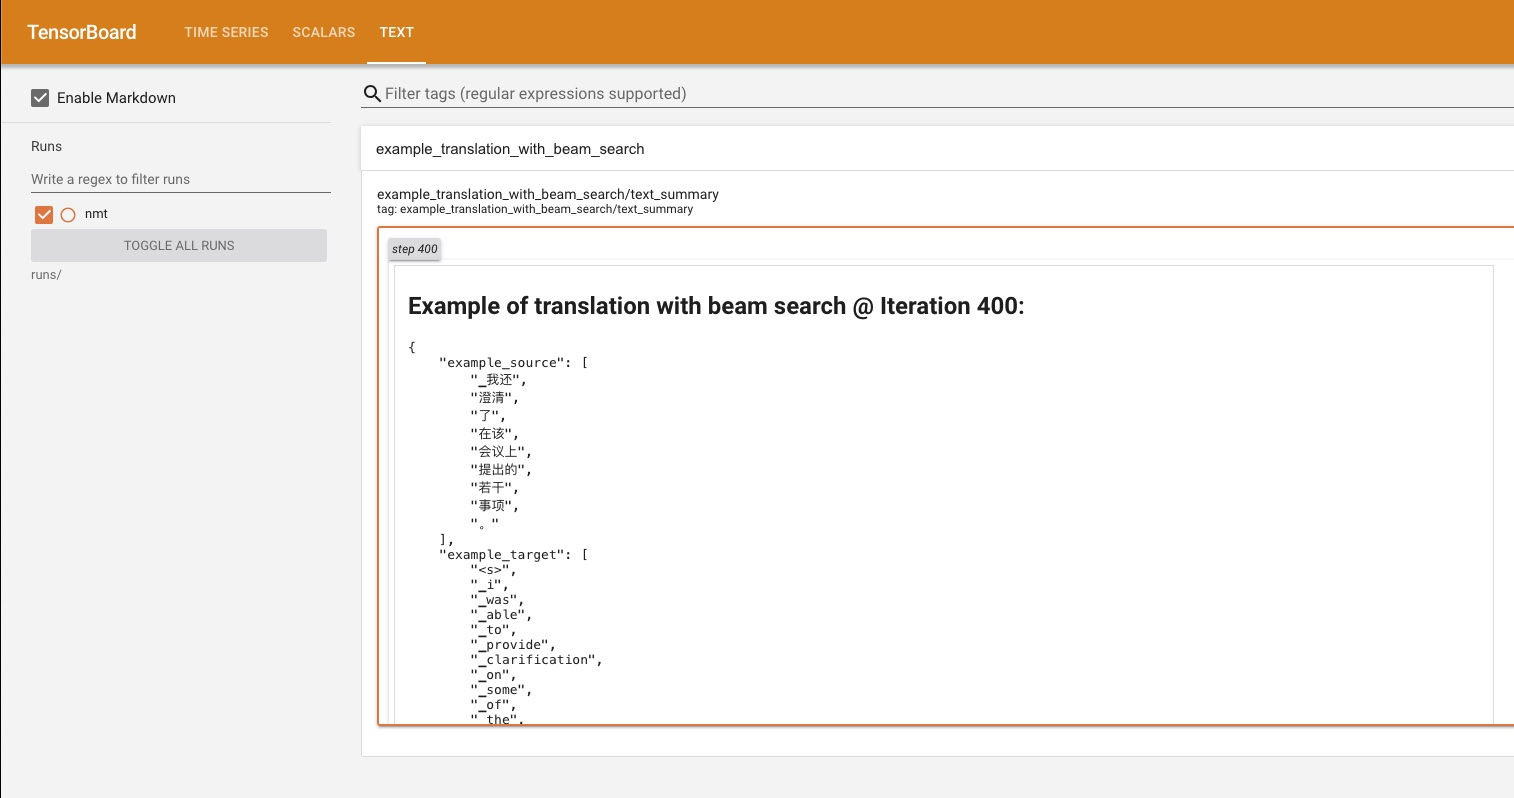
\includegraphics[width=0.7\textwidth]{images/example_translation_beam.jpg}
        \caption{Translation with beam search results for an example sentence are recorded in tensorboard for various iterations. The same data is available in the \texttt{outputs/beam\_search\_diagnostics/} folder in your working directory.}
        \label{fig:beam-search-diagnostics-tensorboard}
    \end{figure}
    

\end{parts}
